%\addcontentsline{toc}{chapter}{Development Process}
\chapter{Design}
This chapter will give an overview of the design of the final system, however will not go into much detail for individual parts of the system. Those designs are within the next chapter as design took place within each iteration rather than at the start.
TODO: could this chapter actually be after the Iteration chapter?
\section{Overall Architecture}
\subsection{System Interaction Diagram}

\section{Database Design}
\begin{sidewaysfigure}
	\caption{Entity relationship digram for final database}
	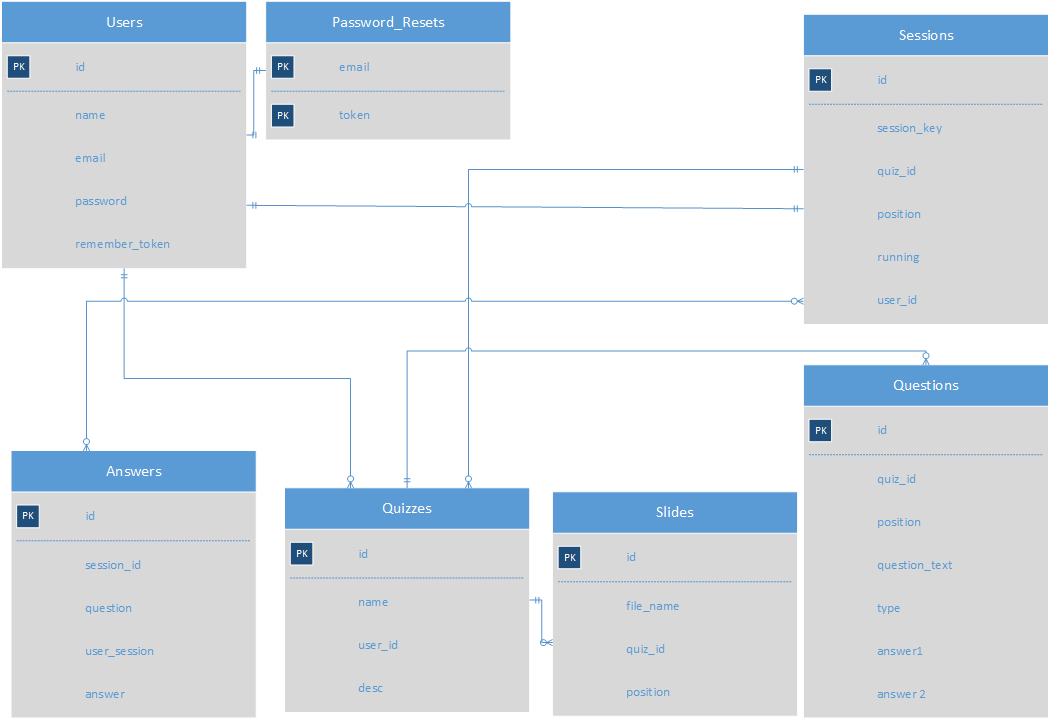
\includegraphics[width=\textwidth]{Chapter2/Final-ER-Image}
	\label{fig:er-diagram}
\end{sidewaysfigure}
\newpage

There are seven tables within the application. Two of these were generated by running a Laravel command to make the authentication part of the site, the users and password\_resets tables. These provide basic user login.

The quizzes table contains information about the quizzes themselves, and are associated with a user. The questions and slides tables both store information about their respective parts of a quiz, with each row within these tables associated with a quiz. Questions store information about the actual question including all the answers, not in the design above are the other eight fields for answers up to answer10. The slides table stores the file name of a slide image that has been converted from a pdf slide. Both of these tables store the positions of their items within a quiz.

The sessions table stores the information about the runnable session, each user has one associated session row. Within this row, the session\_key is stored, which is the key that students would use to connect to a session. Additionally it stores information about the session when its running, specifying if it is running, and what position it is at. This position references the positions specified int he questions and slides tables, though there is no actual foreign key relationship between them. 

The final table, answers, stores all the responses from users to questions. It stores which question, the answer given and the user that submitted the answer. The user\_session is a cookie value rather than a user from the database.